\chapter[Estado do arte]{Estado do Arte\label{estado_do_arte}}

Neste capítulo explicarase como funciona a internacionalización e localizacion con GNU Gettext. Ademais analizaremos as diferentes alternativas que existen no mercado como ferramentas de asistencia a tradución e as caracteristicas que cada unha incorpora. O final faremos un resumo das características que empregan os programas CAT\footnote{Computer Assisted Translation}.

\section{Internacionalización é localización con GNU Gettext}
Gettext é un sistema para a internacionalización e localización amplamente usado en entornos UNIX. Conta con varías implementacións, sendo a primira de Sun Microsystems no ano 1990. A implementación máis usada é a que GNU liberou no ano 1995. Pese ser unha solución antiga, é a día de hoxe a mellor que se pode atopar no mercado.

Para internacionalizar un programa con GNU Gettext non empregaremos as cadeas de texto directamente como podería ser no seguinte program de exemplo:

\begin{lstlisting}[language=C,label=some-code,caption=Some Code]
#include <stdio.h>

int
main ()
{
    printf ("Hello World!");
}
\end{lstlisting}

En lugar diso chamaremos a unha función especial que proporciona Gettext de nome \lstinline{gettext()} pero que é máis empregada a través do seu alias \lstinline{_()}. Ademais configuraremos o programa para que colla a tradución do idioma que queiramos. Desta forma o programa anterior quedaría:

\begin{lstlisting}[language=C,label=some-code,caption=Some Code]
#include <stdio.h>
#include <libintl.h>

#define _(str) gettext(str)

int
main ()
{
    setlocale (LC_ALL, "");
    bindtextdomain ("helloworld", "/usr/local/share/locale");
    textdomain ("helloworld");

    printf (_("Hello World!"));
}
\end{lstlisting}


As súas principais caracteristicas son:

\paragraph{Soporte de plurales}
Algo que pode parecer trivial como o soporte de plurales deixa de selo cando consideramos que non todos as linguaxes do mundo empregan dous plurales. A lingua eslovaca, por exemplo, conta con tres formas de plural de forma que o plural faise diferente para 1, 3 e 5 elementos.

Gettext representa a forma de plural de cada linguaxe con unha cadea da seguinte forma: $$nplurals=n; plural=exp;$$ Onde $n$ representa o número de plurais da linguaxe e $exp$ a expresión para calcular cando debemos empregar cada forma.

\paragraph{Gardado dos orixes das cadeas}
Gettext almacena para cada cadea en que lugares do código aparece esta. O cal pode ser moi interesante para implentar a previsualización das traducións.

\paragraph{Comentarios dos programadores}
É unha función moi importante xa que en moitas ocasións nas linguaxes a mesma palabra empregase como verbo ou como nome polo que en ocasións é importante incorporar un contexto para esa tradución.

\paragraph{Comentarios dos traductores}
A biblioteca permite que os traductores comenten as cadeas.

\section{Ferramentas CAT do mercado}

Nesta sección repasaremos as alternativas existentes no mercado.

\subsection{GTranslator}
GTranslator é a aplicación oficial do proxecto GNOME para a asistencia a tradución. Este aplicativo so permite a tradución de arquivos GNU Gettext. As caracteristica máis destacables deste programa son a posibilidade de abrir varios ficheiros en diferentes lapelas, soporte de memorias de tradución, perfiles para diferentes traductores, edición dos comentarios dos ficheiros .po e un sistema de plugins que permite extender a ferramenta.

\begin{figure}[h]
    \centering
    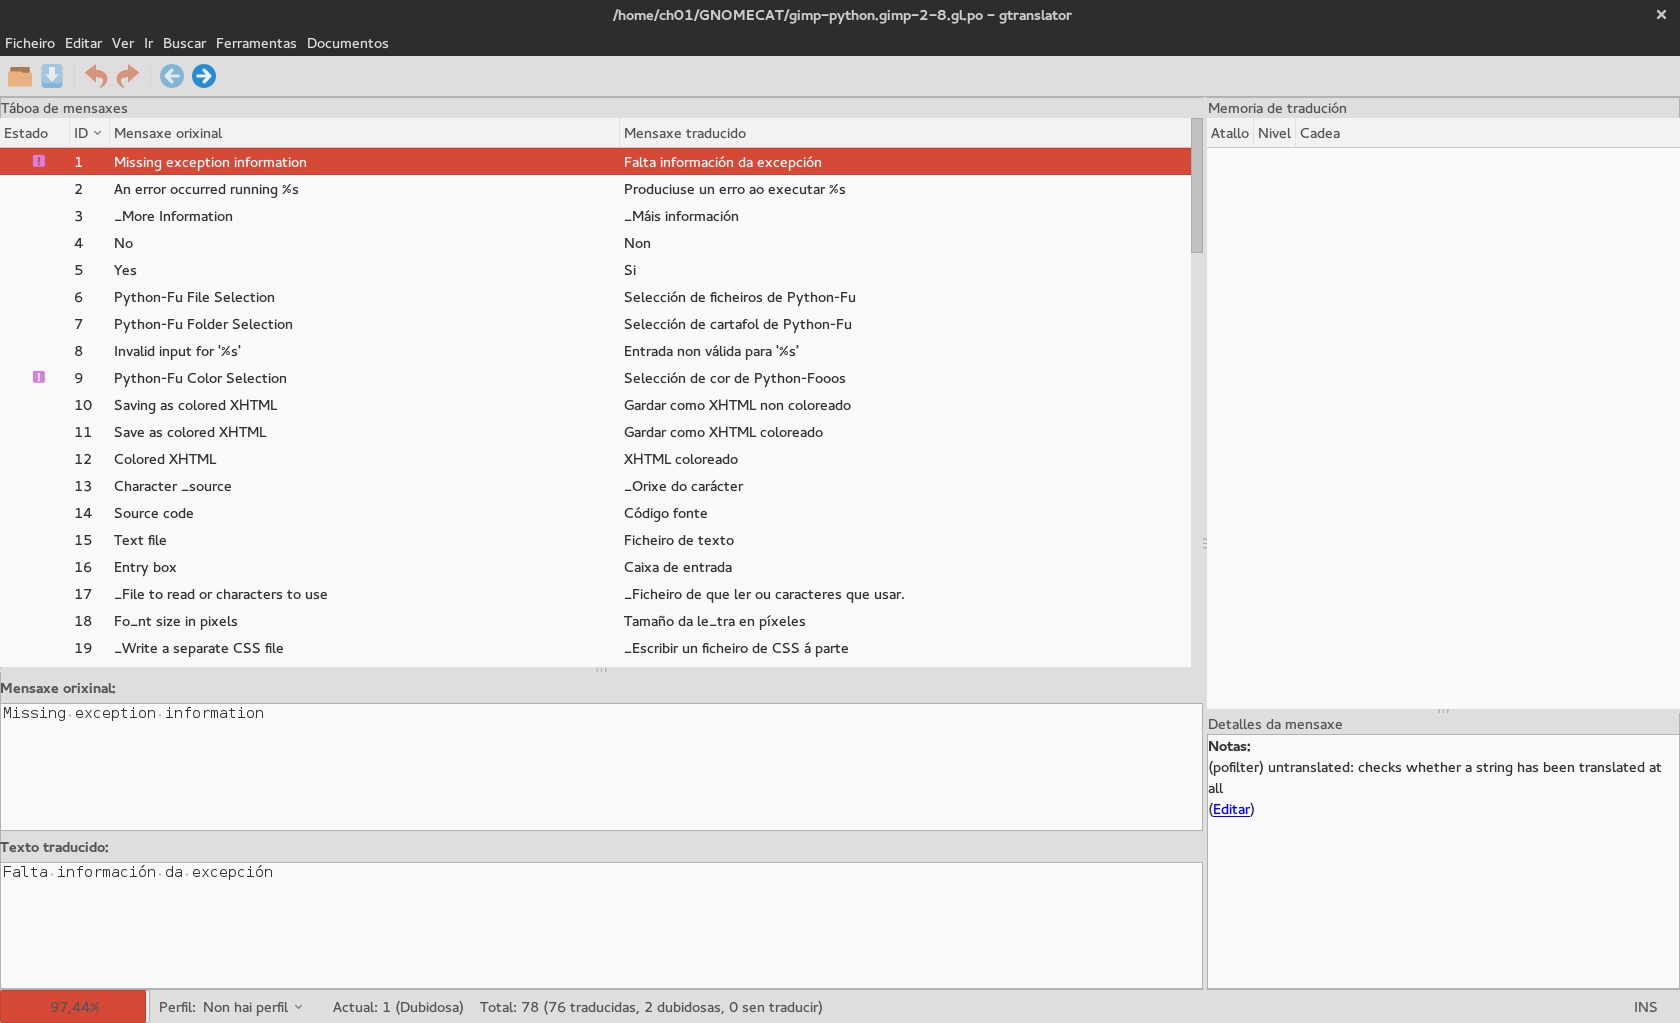
\includegraphics[width=\textwidth]{img/captura_gtranslator.png}
    \caption[Interface de GTranslator]{Interface de GTranslator}
    \label{fig:gtranslator}
\end{figure}

En canto a interface, podemos ver que a parte máis importante do programa é a a lista de mensaxes. Abaixo temos un panel onde podemos editar cada mensaxe e a dereita a memoria de tradución. O programa tamén incorpora atallos de teclado que permiten moverse polo documento e selecionar cada elemento da memoria de tradución.

\subsection{Lokalize}
Lokalize é o programa oficial para a tradución en KDE. Ten soporte para ficheiros GNU Gettext e para Qt ts (o formato propio de KDE) entre outros. Entre as caracteristicas a destacar é o soporte para proxectos de tradución cunha panel resumo de tod o contido de cada proxecto, ten glosario, memoria de traducion, posibilidade de ver os propios ficheiros fonte desde a interface a través de scripts feitos polo traductor, multiples perfiles, etc.

\begin{figure}[h]
    \centering
    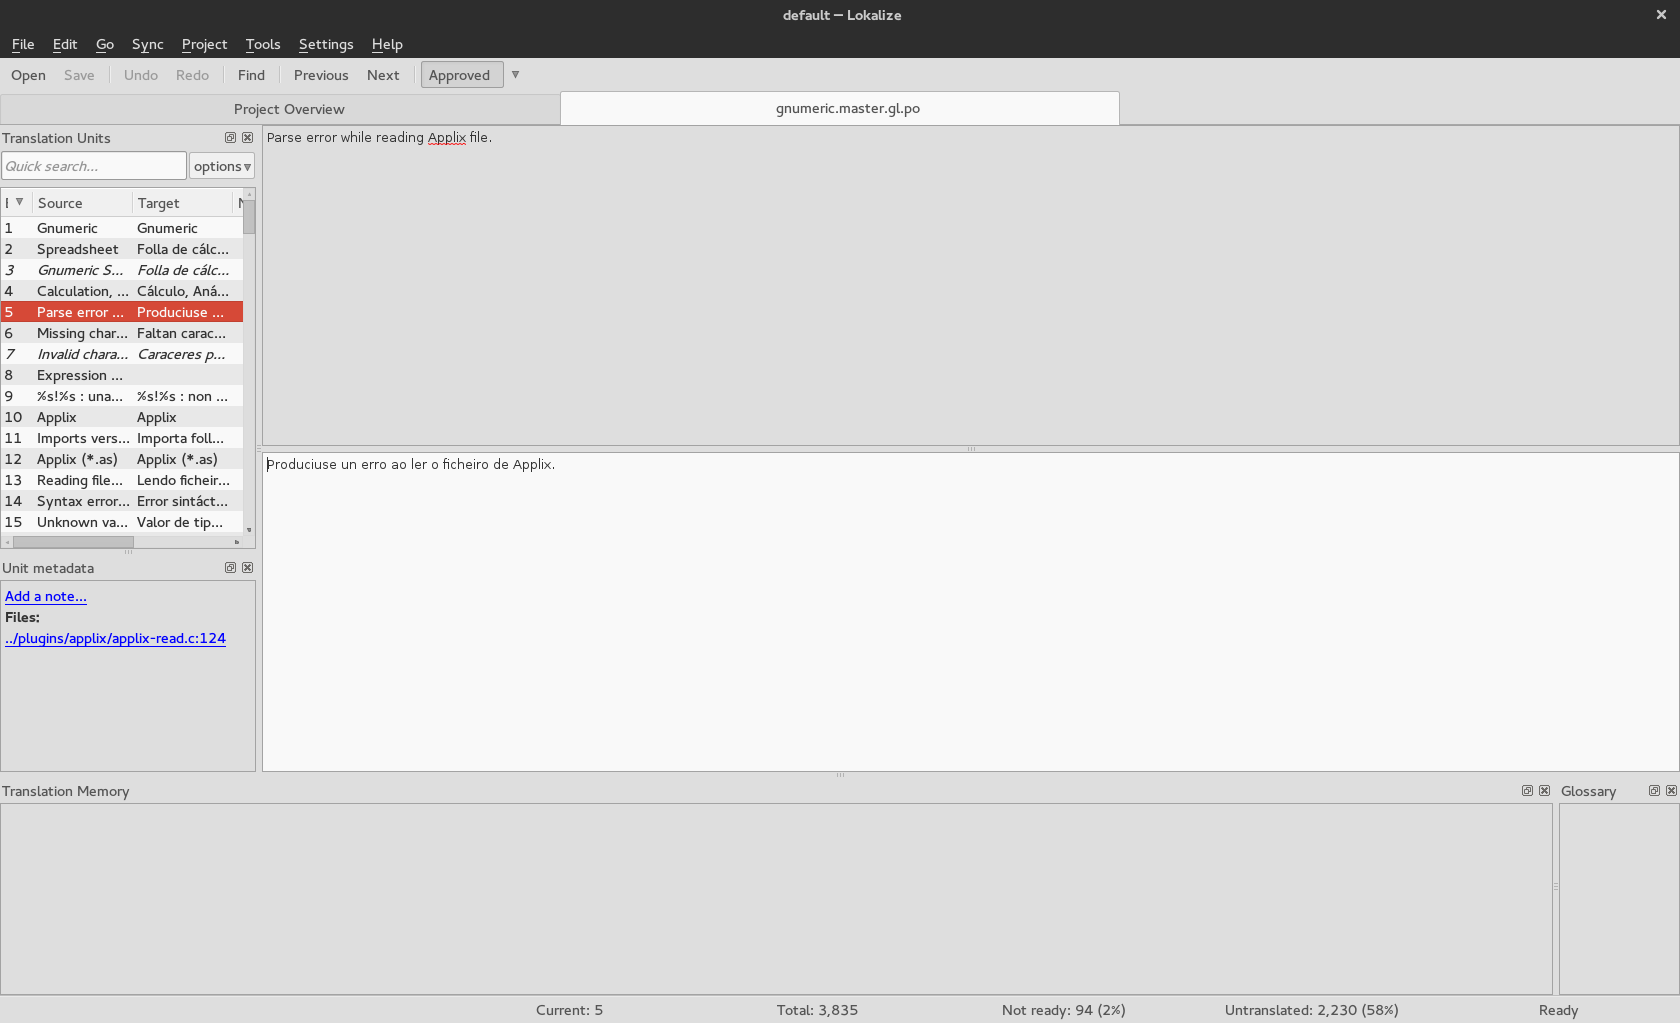
\includegraphics[width=\textwidth]{img/captura_lokalize.png}
    \caption[Interface de Lokalize]{Interface de Lokalize}
    \label{fig:gtranslator}
\end{figure}


\subsection{Virtaal}

\subsection{OmegaT}

\subsection{Google Translation Toolkit}
Metras que todas as solucións anteriores eran solucións de escritorio, Google Translation Toolkit é unha ferramenta web desenvolvida por Google.

\subsection{Transifex}
Tamén se trata dunha solución web. Neste caso de pago.


%
% FIN DEL CAPÍTULO
%